%\addcontentsline{toc}{chapter}{Kapitel-1}
\chapter{Bibliotheken/Software \label{kap1}}

In diesem  Abschnitt werden einige Möglichkeiten zur Erkennung von Partikeln in einem Video niedriger Auflösungsqualität verglichen. Es wäre natürlich ideal einen Vergleich zwischen manuellen und werkzeugbasierten Erkennung zu ziehen. Aber leider wird die manuelle Erkennung hier nicht vollzogen aufgrund der viel zu schwierig bzw. langwierige Arbeit, die sie bereitet. Es geht hier nämlich um mehrere hunderte von Partikeln pro Bild.\\
 
\begin{figure}[H]
    \centering
    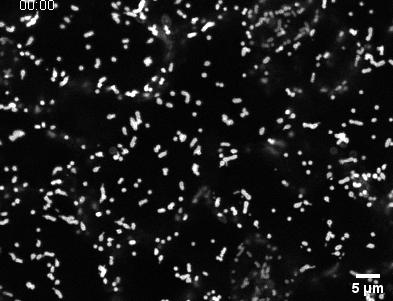
\includegraphics[scale=0.9]{Grafiken/trackpyBilder/video-frame00001.png}
    \caption{Rohbild mit zu erkennenden Partikeln.}
    \label{fig:kap1_rohbild}
\end{figure}

In diesem Sinne widmet sich die Arbeit in der Folgezeit dem Vergleich möglicher Tools, die zur Erreichung der eigentlichen Ziele benutzt werden können. Hierbei werden aus der Vielzahl der Tools nur vier herausgegriffen. Diese werden dann einer textuellen Analyse der Unterschiede unter ihnen unterzogen.\\

Es ist jedoch unerlässlich, hier zum besseren Verständnis der Arbeit zu erwähnen, dass die meisten der im Folgenden betrachteten Bibliotheken Bibliotheken sind, die es ermöglichen, Partikel durch ein Video hindurch zu verfolgen. Da das Verfolgen von Partikeln ein Schritt nach der Erkennung ist, haben wir uns dafür entschieden, mit Bibliotheken zu arbeiten, die das Verfolgen von Partikeln ermöglichen. Wir haben uns auf die Verfolgung von Partikeln konzentriert, da es gewusst ist, dass die Verfolgung erst nach der Erkennung erfolgt. Genauer gesagt, weil das Tracking das Produkt einer Reihe von Erkennungsvorgängen im Verlauf eines Videos ist.
Auf diese Weise möchten wir Missverständnisse ausräumen, die durch die Verwendung des Begriffs `\textbf{Tracking/Verfolgung}' und nicht `\textbf{Erkennung}' entstehen könnten.  

%\todo{ Completer le tableau}
%
%\begin{tabular}{|c||c|c|c|c|}
% \hline
% Werkzeug & Tutorials & Zugänglichkeit & Parametrisierbarkeit & Dokumentation \\
% \hline
% \hline
% ParticleTracker & +++ & ++ & ++ & +++\\
% \hline
% STracking & ++ & + & + & ++\\
% \hline
% STP  & -- & - & + & --\\
% \hline
% TrackPy  & ++++ & ++ & + & ++++\\
% \hline
%\end{tabular}
%\\

%\todo{\href{file:///C:/Users/leb/Downloads/10.21105.joss.04398.pdf}{MyPTV}, \\ \href{https://www.sciencedirect.com/science/article/pii/S2001037021002944}{PySTACHIO},\\ \href{https://spt.readthedocs.io/en/latest/}{SPT}
%\\ \href{https://www.google.com/search?q=Python+package+for+particle+tracking&rlz=1C1CHBF_deDE987DE987&sxsrf=ALiCzsYl2NtGnlFYYupES17uNyNLp8zhIQ:1653590912505&ei=gMuPYoKwHsyMxc8Phquk2AM&start=10&sa=N&ved=2ahUKEwiC8MWX6v33AhVMRvEDHYYVCTsQ8NMDegQIARBQ&biw=1920&bih=969}{Python package for particle tracking}}

\section{ParticleTracker \label{kap1_ParticleTracker}}
\textbf{ParticleTracker} ist eine vollständig grafisch bedienbare Software, die es erlaubt, Partikel aus einem Video guter oder niedriger Auflösung zu verfolgen. Diese verwendet mehrere verschiedene Verfolgungsalgorithmen mit einer Standardschnittstelle, um die Einrichtung verschiedener Partikelverfolgungsprojekte schnell und einfach zu gestalten \cite{Smith2021}.
Es verwendet drei verschiedene Methoden/Funktionen zur Erkennung von Partikeln in einem Video. Alle diese Methoden haben ihre eigenen Besonderheiten bei der Verwendung, nämlich:
\begin{itemize}
   \item \textit{Opencv Hough Circles}:\\ Es ist eine Methode, die von OpenCV\cite{opencv_library} entwickelt und zur Verfügung gestellt wurde. Diese Option wurde hauptsächlich für die Erkennung von Objekten entwickelt, die kreisförmig aussehen oder eine kreisförmige Form haben. Dies ist in unserem Fall nicht sehr interessant, da die in unserem Video gezeigten Partikel verschiedene Formen haben können (kreisförmig, quadratisch, längs und ...). Allerdings verwendet sie nicht die klassische \textbf{Hough Transform}\footnote{Es ist eine von vielen Methoden, um einen Kreis in einem Bild zu erkennen.}, die in ``THE STANDARD HT'' \cite{comparative_hough_transform} und ziemlich zeitaufwendig und speicherkostend ist, da sie die Suche nach drei Unbekannten/Parametern erfordert, wie die mathematische Darstellung des Kreises unten zeigt:\\
\begin{center}
 $(x- x_{center})^{2} + (y - y_{center})^{2} = r^{2}$ \\
\end{center}
Wobei $(x_{center},y_{center})$ ist der Mittelpunkt des Kreises.\\
      $r$ ist der Radius des Kreises.\\
      

Stattdessen wird der \textbf{Hough Gradient} (im Wesentlichen beschrieben in `21HT'' \cite{comparative_hough_transform}) verwendet,der die Informationen des Gradienten\footnote{``The gradient is the generalization of the derivative to multivariate functions. It captures the local slope of the function, allowing to predict the effect of taking a small step from a point in any direction.'' — Page 21, Algorithms for Optimization, 2019 \cite{algo_optimi_2019}.} berücksichtigt.
      
   \item \textit{Trackpy}:\\ Diese Methode ist nach der Bibliothek benannt, die sie entwickelt und zur Verfügung gestellt hat, nämlich: trackpy.  Trackpy ist eine Bibliothek zur Verfolgung von Partikeln in 2D, 3D und höheren Dimensionen. Weitere Informationen zu dieser Bibliothek liefern wir in einem gesonderten Abschnitt dieser Arbeit.
   
   \item \textit{Opencv Contour finding}:\\ Ist auch, wie der Name schon sagt, eine OpenCV-Methode mit dem Ziel, Konturen\footnote{Eine Kontur kann einfach als eine Kurve interpretiert werden, die alle aufeinanderfolgenden Punkte (entlang des Grenzbereichs) mit derselben Farbe oder Intensität verbindet. Konturen sind nützliche Werkzeuge zur Analyse von Formen und zum Erkennen und Identifizieren von Objekten.} in einem Binärbild\footnote{Ein binäres Bild ist ein Bild, dessen Pixel nur zwei mögliche Intensitätswerte haben. Numerisch sind diese beiden Werte meist 0 für Schwarz, 1 oder 255 für Weiß.} zu finden.Die Funktion ruft die Konturen des Binärbildes ab, indem sie den Algorithmus \cite{topological_contour_finding} verwendet. Konturen sind ein nützliches Werkzeug für die Musteranalyse und das Erkennen und Erfassen von Objekten.
\end{itemize}

    \paragraph{Ein-/Ausgabe \\} 
    Als Eingabe akzeptiert ParticleTracker Videos in fast allen gängigen Formaten wie avi, mp4, MOV etc... .\\

Jedoch gibt es bis zu drei Möglichkeiten für die Ausgabe. Diese sind wie folgt:
\begin{itemize}
\item \textit{DataFrame}\footnote{Ein DataFrame ist eine Datenstruktur in Python, die Daten in einer 2-dimensionalen Tabelle mit Zeilen und Spalten organisiert, ähnlich wie eine Tabellenkalkulation.}: Dieser Datenrahmen enthält die Werte aller im Video vorhandenen Partikel im Laufe der Zeit. Er enthält in der Reihenfolge Frame (Frame-Nummer), x(Position auf der x-Achse), y(Position auf der y-Achse), mass(Helligkeit), size, ecc, raw\_mass, ep, particle, user\_rad

\item \textit{CSV}: Liefert ebenfalls die gleichen Ergebnisse wie beim DataFrame, allerdings im csv-Format

\item \textit{Video}: Hier handelt es sich um ein neues Video, das aus den Bildern des Videos erstellt wurde, das für die Entdeckungen verwendet wurde. Nur hier bleiben alle erkannten Partikel, die eingekreist und/oder nummeriert wurden, im gesamten (neuen) Video so eingekreist/nummeriert.
\end{itemize}



	\paragraph{Vorteile}
		\begin{enumerate}
    			\item \textbf{GUI bedienbar}: \\
				Die Benutzeroberfläche ist eine angenehme Arbeitsmethode  für Benutzer, insbesondere für Neulinge (Siehe \cite{hertzum1996browsing}). Dies ist sicherlich eine hervorragende Möglichkeit, in diesen Bereich einzusteigen, ohne sich mit zu vielen Codezeilen auseinandersetzen zu müssen oder Programmierkenntnisse zu besitzen.
				
    			\item \textbf{Anfängerfreundlich}:\\
				Die Anfängerfreundlichkeit ist stark auf den vorherigen Punkt zurückzuführen, nämlich die GUI-Bedienbarkeit. Zudem ist es sonderlich umstandslos, mit Hilfe einiger Klicks, sich Informationen(x(Position auf der x-Achse), y(Position auf der y-Achse), mass(Helligkeit), size, ...) über jedes Partikel in jedem Bild generieren zu lassen, die relevant sind.    
				
    			\item \textbf{Datenvisualisierung}:\\
    			Ein großer Vorteil ist Datenvisualisierung. Dies liegt an der schrittweisen und automatischen Aktualisierung des Renderings(Anzeige der Ergebnisse der Partikelerkennung auf dem Bild.) in Abhängigkeit von den vorgenommenen Einstellungen.% Allerdings ist es notwendig, zunächst das Kästchen "Annotate" zu aktivieren, um die Live-Ansicht zu aktivieren.
    			
    			\item \textbf{Datenausgabe}:\\
 				Der Zugang zu den Daten in der Software ist schnell und einfach. Außerdem sind die Daten in verschiedenen Formen verfügbar. Unter anderem werden die Daten als csv-Datei und auch als Video bereitgestellt, das den Fortschritt der erkannten Objekte/Partikel im Ausgangsvideo nachzeichnet. 
Es ist auch wichtig zu erwähnen, dass es möglich ist, die Daten (in csv) in Bezug auf ein einzelnes Bild zu exportieren.
		\end{enumerate}
		
	\paragraph{Nachteile}
		\begin{enumerate}
				\item \textbf{Das Hochfahren der Software}:\\
				Trotz der Dokumentation war es nicht einfach, die Software zum Laufen zu bringen. In Anbetracht der Verwendung von Bibliotheken, die nur in einer bestimmten Python-Umgebung  verfügbar sind, nämlich `Conda'\footnote{Conda ist ein Open-Source-Paketverwaltungssystem und Umgebungsverwaltungssystem, das auf unter Windows, macOS und Linux läuft ausgeführt wird. Es ermöglicht die schnelle Installation, Ausführung und Aktualisierung von Paketen und deren ihren Abhängigkeiten.}.
Daher wäre es fair zu erwähnen, dass dies für Laien noch schwieriger sein könnte.
				
    			\item \textbf{Funktionsbegrenzt}:\\
				Die Benutzung über eine GUI ist zwar ein begeisternder Punkt. Doch genau hier liegt die Schwäche. Da die Benutzeroberfläche bereits konfiguriert ist, bietet sie nur die Möglichkeit, die verfügbaren Optionen zu nutzen. Dies könnte in manchen Fällen zu einem Mangel an Optionen führen und somit unzureichend sein. Es Beispiel hier wäre: Falls man den Wert der verwendeten Parameter jedes Mal ändern möchte, wenn die Anzahl der erkannten Partikel unter einer vordefinierten Anzahl oder sogar unter einem Prozentsatz liegt. 			
    			
    			\item \textbf{Nicht intuitiv}:\\
    			Obwohl die Verwendung einer grafischen Oberfläche im Allgemeinen für den Benutzer attraktiver ist, sollte sie so intuitiv wie möglich sein oder gut dokumentiert werden (zumindest als Tooltip).
In diesem Fall sind die Namen einiger Optionen auf der Schnittstelle nicht sehr aussagekräftig oder beschreibend(siehe \ref{fig:kap1_PT_Nicht_Intuitiv}).
\begin{figure}[H]
    \centering
    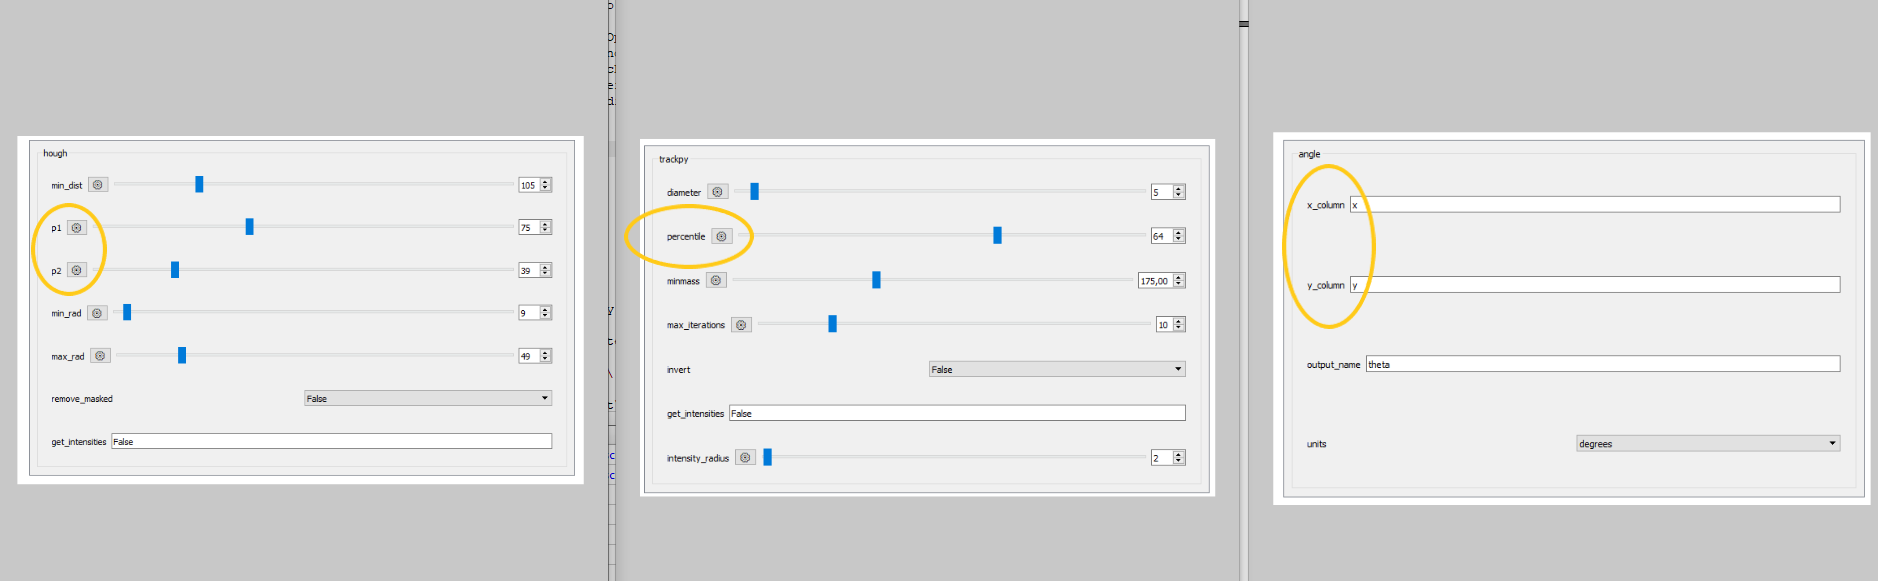
\includegraphics[scale=0.35]{Grafiken/particletracker/Not intuitive.png}
    \caption{Unzureichend beschriebene Optionsnamen}
    \label{fig:kap1_PT_Nicht_Intuitiv}
\end{figure}
Es ist daher verständlich, dass man Hinweise erwartet, die die Verwendung der Optionen (Schaltflächen) im Detail beschreiben. 
Dies ist leider nicht der Fall. Daher erfordert die Benutzung der Software ein gewisses Hin und Her in der externen Dokumentation, um die Rolle der Optionen zu lernen.
\end{enumerate}
		
	\paragraph{Beispiel\\}
	Wir zeigen hier ein Beispiel für die Erkennung von Partikeln auf einem bestimmten Bild.
	 
	\begin{figure}[H]
    \centering
    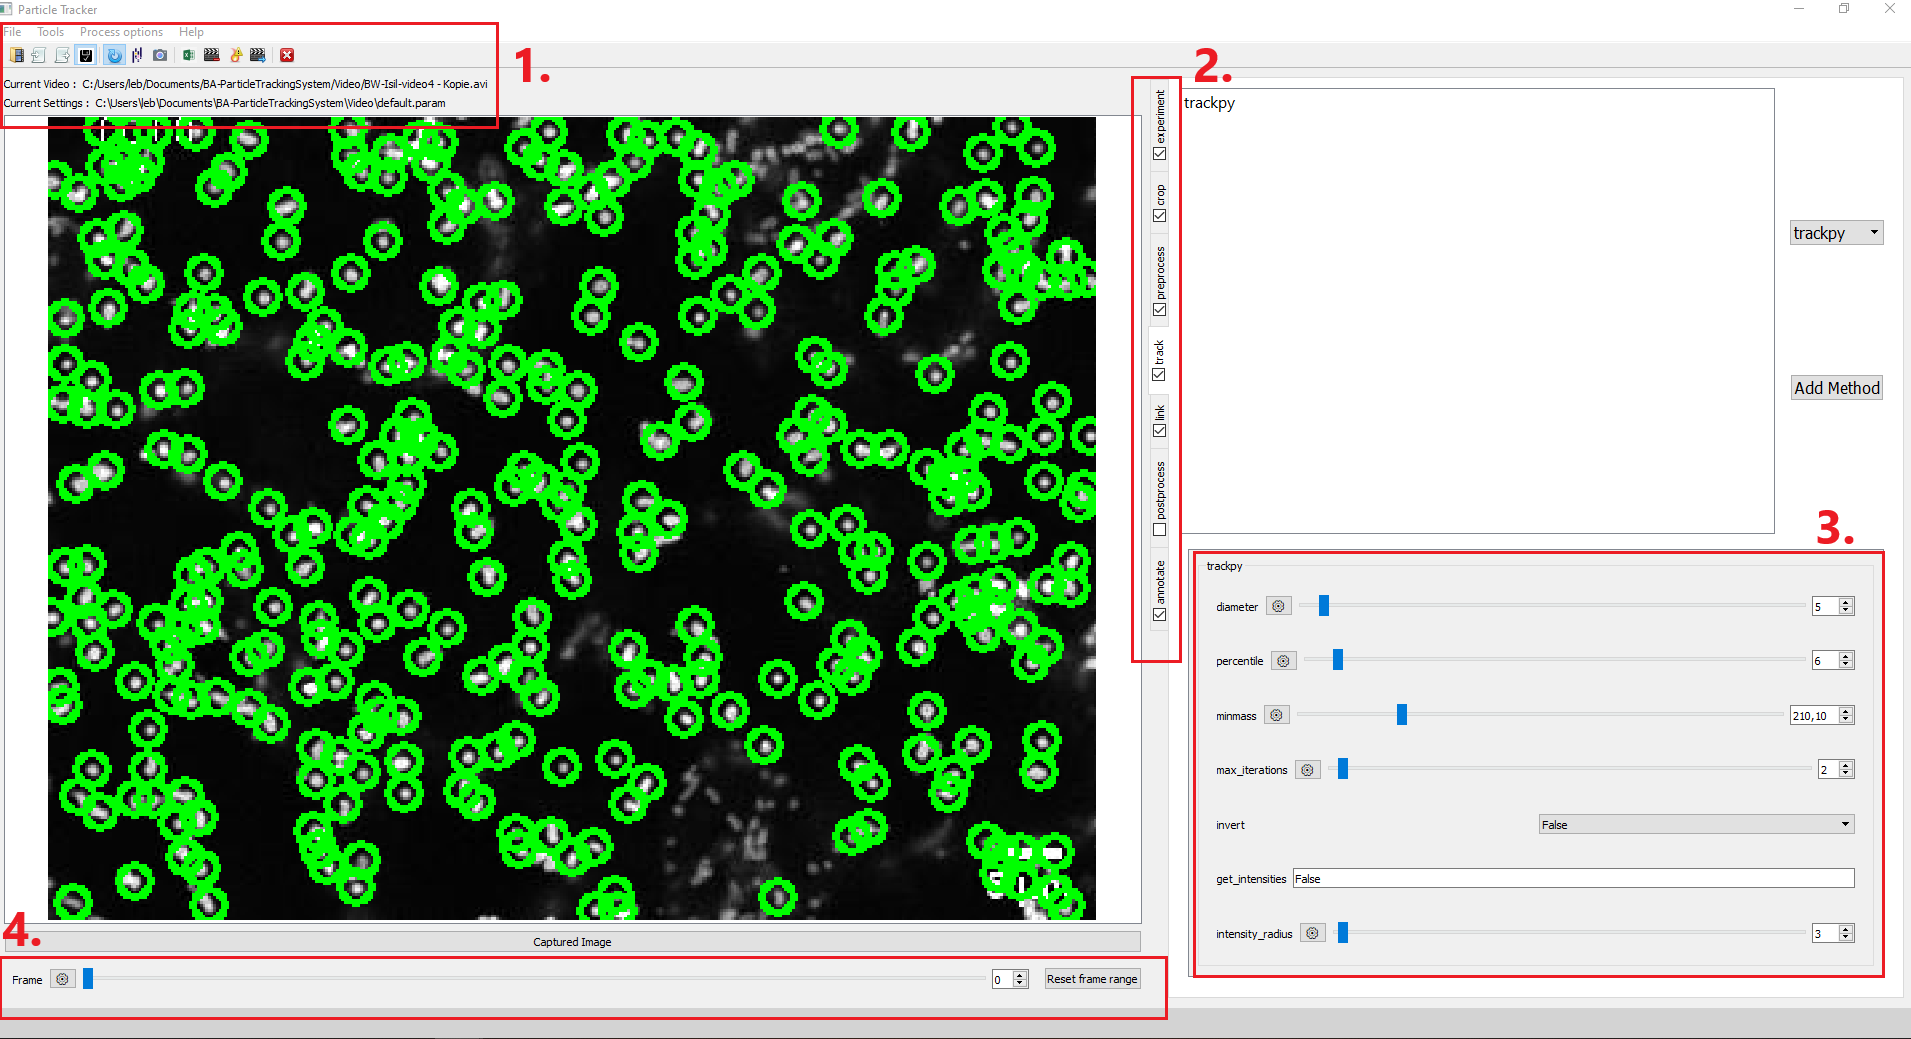
\includegraphics[scale=0.3]{Grafiken/particletracker/Using trackpy.png}
    \caption{Beispiel einer Partikelerkennung mit der Trackpy-Methode von ParticleTracker.}
    \label{fig:kap1_PT_Beispiel}
\end{figure}

\begin{tabular}{|l|p{12cm}|}
\hline
\texttt{1.} & Hier geht es um alles, was mit der Eingabe und Ausgabe von Daten zu tun hat. \\ \hline
\texttt{2.} & Es geht hier um die Optionen, die angewendet/aktiviert werden müssen, um im Rendering-Bereich (Bereich direkt unter 1.) angezeigt zu werden. \\ \hline
\texttt{3.} & Hier können die Werte der Parameter für die Lokalisierung geändert werden. \\ \hline
\texttt{4.} & Es zeigt das Bild, auf dem man sich gerade befindet. \\ \hline
\hline
\end{tabular}

Auf diesem Bild sehen wir eine Menge kleiner grüner Kreise, die kleine weiße Partikel umschließen. 
Es ist zu erkennen, dass die meisten dieser weißen Partikel eingekreist sind. Das bedeutet in diesem Fall, dass sie entdeckt wurden. Daher scheint die Erkennung hier ziemlich gut zu sein. Obwohl sie einige Partikel redundant zu erfassen scheint.


\newpage
	
\section{STracking}
\textbf{STracking} ist ein Framework, dessen Ziel es ist, eine Pipeline\footnote{Ein Verfahren, das es ermöglicht, die verschiedenen Schritte der Verarbeitung eines Befehls durch den Prozessor voneinander unabhängig zu machen.} für die Partikelverfolgung zu entwickeln. Diese Pipeline besteht aus folgenden voneinander unabhängigen Schritten:
\begin{itemize}
\item Frame-by-Frame Partikelerkennung
\item Partikelverknüpfung
\item Analyse von Partikeleigenschaften 
\item Entwurf von Track-Features
\item Filterung von Tracks
\end{itemize}

Es stellt drei Methoden zur Verfügung, um die Partikelerkennung und -verfolgung durchzuführen, die jeweils auf spezifischen Algorithmen basieren, nach denen sie benannt sind.  Wir haben namentlich:

\begin{itemize}
	\item \textbf{Difference of Gaussians (DoG)}: ist ein Algorithmus zur Verbesserung von Graustufenbildern, bei dem eine unscharfe Version eines Originalgraustufenbildes von einer anderen, weniger unscharfen Version des Originals subtrahiert wird \citep{DoG_1}.
	
	\item \textbf{Determinant of Hessian (DoH)}: Der als solche funktioniert, wie im Artikel von \textit{Jan Sellner (2017)} "\textit{Introduction to the Hessian feature detector for finding blobs in an image}'' \cite{DoH_sellner_2017} dargestellt,\\ `\textit{An image is scaled to a size defined by the scale parameter $\sigma$. Let \textbf{$H_{\sigma}$} denote the Hessian matrix at a specific image location in level \textbf{$\sigma$} and e.g. \textbf{{\large $\partial_{xx} = \frac{\partial^{2}I}{\partial^{2}x^{2}}$}} denoting the second order derivative of the image $I$ along the $\textbf{x}-axis$. We can use the normalized determinant response of the Hessian 
	\begin{center}
	 \textbf{{\large $\sigma ^{4} \cdot det(H_{\sigma}) = \sigma ^{4} \cdot (\partial_{xx} \cdot \partial_{yy} \cdot \partial^{2}_{xy})$}}\\
	 \end{center} 
to detect image features (blobs and notches) by searching for maxima in each image location across scale.}' \cite{DoH_sellner_2017}	
	
	\item \textbf{Laplacian of Gaussians (LoG)}: Er hebt Regionen mit schnellen Intensitätsänderungen hervor und wird daher häufig zur Kantenerkennung verwendet \cite{LoG_1}. 
\end{itemize}

Obwohl es für jede Anwendung zur Verfolgung von Punkten in 2D+t- und 3D+t-Bildern verwendet werden kann, ist seine Hauptidee die Verfolgung intrazellulärer Objekte (alle Objekte/Partikel, die innerhalb einer Zelle sind) in Mikroskopiebildern. Sowohl in 2D+t (2-Dimension nämlich x-position und y-position) als auch in 3D+t (3-Dimension nämlich x-position, y-position und z-position) \cite{prigent_2020}. Wobei t für Zeit steht.\\
In Kombination mit dem Plugin \textbf{napari}\cite{prigent_2021_napari} bietet es die Möglichkeit, den Tracking-Prozess über eine grafische Benutzeroberfläche zu verwalten.


\paragraph{Ein-/Ausgabe \\} 
    STracking verwendet als Eingabedaten Bilder oder Sequenzen von Bildern im TIFF-Format\footnote{ist eine Computerdatei, die zum Speichern von Matrixgrafiken und Bildinformationen verwendet wird} (Abkürzung für Tag Image File Format). Daneben ist es auch möglich, den Inhalt von csv-, xml- und StIO-Dateien zu lesen.\\

In Bezug auf die Ausgabe bietet es die Möglichkeit, die Ergebnisse in verschiedene Formate zu exportieren, nämlich:
\begin{itemize}
\item \textit{csv}: Unterstützt keine Aufspaltungs- (Ereignis, bei dem ein Partikel sich in mehrere splittet) und Fusionsereigniss (Ereignis, bei dem mehrere Partikeln zusammenführen),
\item \textit{StIO}: Dieses Format wurde von STracking entwickelt, um die Daten leichter speichern zu können.
\end{itemize}

	\paragraph{Vorteile}
		\begin{enumerate}
    			\item \textbf{Leicht installierbar}:\\
				Mit den in der Dokumentation beschriebenen Schritten ist es relativ einfach, die Bibliothek zu installieren. Die Dokumentation erwähnt Wege, wie die Installation durchgeführt werden könnte, nämlich über \textit{PyPI} und/oder über die \textit{Das Herunterladen und Installieren des Quellcodes über git.}

    			\item \textbf{GUI bedienbar}:\\
				Wie erwähnt ist es möglich, das Programm über eine grafische Benutzeroberfläche zu verwenden. Dies geschieht nach der Installation des napari-Plugins.
Hier müssen die ersten Schritte jedoch per Code gemacht werden. 
Das Plugin kann also sowohl zur Manipulation als auch zur Visualisierung der Ergebnisse verwendet werden. 
		\end{enumerate}
		
	\paragraph{Nachteile}
		\begin{enumerate}
    			\item \textbf{Lückenhafte Dokumentation}:\\
				In der Tat ist die Dokumentation in Bezug auf die Installation der Bibliothek nicht vollständig. Zum Beispiel wird nirgends erwähnt, dass \textbf{pyQt}\footnote{PyQt ist eine Bibliothek, die die Verwendung des Qt-GUI-Frameworks in Python ermöglicht.} installiert werden muss. Obwohl dieses \textbf{Modul(pyQt)} zwingend erforderlich ist, wenn man die grafische Benutzeroberfläche verwenden möchte.
				
    			\item \textbf{Unerwartete Reaktion der grafischen Benutzeroberfläche}:\\
				Im Gegensatz zu dem, was in der Dokumentation unter dem Punkt `Example 1: Stracking workflow' beschrieben ist, schließt sich das Fenster, das die visuelle Darstellung der Tracking-Aktionen anzeigen soll, automatisch, sobald es geöffnet wird.  Dies ermöglicht natürlich weder das Betrachten noch das Manipulieren der grafischen Darstellung. Es ist wichtig zu erwähnen, dass pyQt in der gleichen virtuellen Umgebung installiert werden muss, um das oben erwähnte Problem zu beheben.
    			
		\end{enumerate}
		

%\newpage	
	
%\section{MyPTV}
%\textbf{MyPTV} \cite{ron_shnapp_MyPTV} ist eine Software, die vorrangig dazu entwickelt wurde, die 3D-Partikel\-geschwindigkeit aufzuspüren. Es handelt sich um eine Open-Source-Software.
%Die Funktionsweise von MyPTV stützt sich stark auf den bewährten mathematischen Rahmen, der im Rahmen des OpenPTV-Projekts (https://www.openptv.net/) entwickelt wurde. Auch die Prinzipien der Photogrammetrie, die in beiden Programmen verwendet werden, sind identisch. Die Software unterscheidet sich jedoch stark durch die Tatsache, dass sie in Python programmiert wurde, das Open Source ist und der wissenschaftlichen Gemeinschaft und nicht-professionellen Computerprogrammierern zugänglich ist.

%	\paragraph{Vorteile}
%		\begin{enumerate}
%    			\item \textbf{Python als Programmiersprache}:\\
%    			Die verwendete Programmiersprache ist Python, wodurch die Software für alle, die sie nutzen wollen, leicht zugänglich ist. Sie bietet ein Computer-Ökosystem, das in der Lage ist, den wissenschaftlichen Anforderungen und Herausforderungen gerecht zu werden \cite{5582063_Python_Ecosystem_Scientific_Computing} .
%Daher ist es interessant, zu erwähnen, dass ein großer Teil der wissenschaftlichen Gemeinschaft aus den oben genannten Gründen Python verwendet. Dies macht Python zur bevorzugten Sprache für Wissenschaftler und Ingenieure \cite{5725235_Python_Scientists_and_Engineers}. 
%
%    			\item \textbf{Breites Spektrum an Möglichkeiten}:\\
%				Die Ressourcen werden so organisiert, dass es für jeden Anwendungsbereich ein spezielles Modul gibt, das alle Funktionen enthält, die in diesem Bereich benötigt werden könnten. So gibt es sechs Module, von der Bildgebung über die Kalibrierung, die Segmentierung, den Partikelvergleich und die 3D-Verfolgung bis hin zum Modul zur Glättung der Pfadlinie.
%    			
%    			
%		\end{enumerate}
%		
%	\paragraph{Nachteile}
%		\begin{enumerate}
%    			\item \textbf{Zielgruppe}:\\
%				Als Software, die speziell für den wissenschaftlichen und engenieurwissenschaftlichen Gebrauch konzipiert wurde, ist sie aufgrund ihrer Komplexität für Laien nicht geeignet.
%				
%    			\item \textbf{Schwer bedienbar}:\\
%				Trotz der vorhandenen Dokumentation ist die Nutzung der Software recht schwierig. Nicht nur, weil sie, wie im vorherigen Abschnitt beschrieben, auf eine bestimmte Gruppe zugeschnitten ist, sondern auch, weil es an einer Anleitung fehlt, die anhand eines trivialen Beispiels Schritt für Schritt die Verwendung der Software zeigt.
%Das macht sie natürlich ziemlich undurchsichtig.
%    			
%		\end{enumerate}
%\newpage

\section{SPT: Single particle tracking analysis \label{kap1_STP}}
\textbf{SPT} \cite{spt_stehr_stein_2020} ist ein Python-Paket, das einen vollständigen Arbeitsablauf für die Analyse der Verfolgung einzelner Partikel bietet. Dabei stützt es sich im Wesentlichen auf andere Pakete wie: \textbf{picasso\_addon} \cite{picasso_addon_schwille-paint_2020} und \textbf{picasso} \cite{picasso_jungmannlab_2019} für die Lokalisierung/Erkennung von Partikeln aus Video und die Analyse von immobilisierten\footnote{Das sind Partikel, die sich während des gesamten Videos überhaupt nicht bewegen.} Partikeln und \textbf{trackpy} \cite{trackpy_allan_daniel_b_2021_4682814} für die Verknüpfung von Lokalisierungen oder die Erstellung von Trajektorien.\\
Die Lokalisierung, die hier die des \textit{Picasso}-Pakets verwendet, konzentriert sich auf einen \textit{gradientenbasierten Ansatz} \cite{soboleva2021raindrops}. Der Gradient oder bzw. die Gradientenkarte wird üblicherweise in der Bildverarbeitung verwendet, um die Kanten von Objekten in einem Bild hervorzuheben.\\ Dabei haben homogene Bereiche eines Bildes meist einen niedrigen Gradienten, der niedriger ist als der Gradient der Objektkanten in demselben Bild. 

\paragraph{Ein-/Ausgabe \\} 
    SPT erlaubt es nur eine einzige Eingabemöglichkeiten,  nämlich Video-Datei. Dabei werden nur zwei Arten akzeptiert: TIFF und binäre Rohdaten (Dateierweiterung ''.raw").\\
    Bei der Datenausgabe bietet SPT eine Reihe von Möglichkeiten, was den Export von Daten angeht: 
    \begin{itemize}
    \item \textit{csv}
    \item \textit{hdf5}
    \item \textit{txt}
    \item \textit{xyz}
    \item \textit{3d}
    \item \textit{roi}
    \end{itemize}
    
    
	\paragraph{Vorteile}
		\begin{enumerate}
    			\item \textbf{Zielgerichtet}:\\
				Wie in seiner Beschreibung angekündigt, stellt er alle Werkzeuge zur Verfügung, die für die Erreichung eines spezifischen Ziels (z.B. Erkennung, Verfolgung oder Trajektorienerstellung von Partikeln) notwendig sind, obwohl er sich auch auf andere Ressourcen stützen kann. Zu Illustrationszwecken verwendet er folgende Tools.
				
				\begin{enumerate}
					\item \textit{picasso}:\\
				 		Für die Lokalisierung und Auswertung von Bildern in verschiedenen Auflösungen.
					\item \textit{picasso\_addon}:\\
						Für alle anderen Funktionen, die neben der Bindung von lokalisierten Partikeln genutzt werden 								können.
					\item \textit{trackpy}:\\
						Für alles, was mit der Verbindung von zuvor lokalisierten Partikeln zu tun hat
				\end{enumerate}
    			
		\end{enumerate}
		
	\paragraph{Nachteile}
		\begin{enumerate}
    			\item \textbf{Schlecht dokumentiert}:\\
				Die Dokumentation des gesamten Handbuchs ist in der Tat sehr unterschiedlich. Sie variiert von sehr wenig Dokumentation für die Installation bis hin zu gar keiner Dokumentation für die Nutzung.  Das macht die Installation und Nutzung natürlich schwierig. Da es immer zu den Paketen navigiert werden muss, die SPT verwendet (nämlich \textit{picasso}, \textit{picasso\_addon} und \textit{trackpy}), um die notwendigen Informationen (zu befolgenden Schritte) für die Installation und gegebenenfalls auch für die Verwendung zu erhalten.
				
    			\item \textbf{Fehlender Benutzerleitfaden}:\\
				Das Fehlen eines Benutzerhandbuchs in einem Paket wie SPT, das sich auf andere Pakete stützt, um Ergebnisse zu liefern, schränkt sowohl die Einarbeitung in die Umgebung als auch deren Beherrschung stark ein. Der Benutzer muss die Funktionen oder Werkzeuge, die er benötigt, selbst aus den Dokumentationen der verschiedenen Pakete lernen und dann zu SPT zurückkehren, um sie anzuwenden.
				
    			
		\end{enumerate}



%\addcontentsline{toc}{section}{Kapitel-1}
%\section{Werkzeugbasierte Erkennung}
\section{Trackpy \label{kap1_trackpy}}
Trackpy ist ein Python-Paket, das es ermöglicht aus einem Video bzw. einer Imagesequenz Partikel in unterschiedlichen Dimensionen (2D und 3D) zu erkennen und zu verfolgen. Hier wird natürlich die Zweidimensionalität anvisiert. Die Erkennung der Partikel erfolgt über eine der Funktionen des Paketes, nämlich die \textit{locate-}Funktion.
Diese verfügt über eine Reihe von Parametern, anhand derer die Qualität der Anerkennung angepasst werden kann.\\

\paragraph{Ein-/Ausgabe \\} 
Trackpy verwendet als Eingabedaten Bilder oder Sequenzen von Bildern. Es kann auch aus Video bestimmter Formate (AVI, MOV, ...) Bildsequenz erstellten und damit arbeiten.\\
In Bezug auf die Ausgabe bietet es die Möglichkeit, die Ergebnisse in verschiedene Formate zu exportieren, nämlich:
\begin{itemize}
\item \textit{csv}  
\item \textit{HDF5}
\item \textit{SQL database}
\item \textit{Excel}
\end{itemize}

	\paragraph{Vorteile}
		\begin{enumerate}
    			\item \textbf{Gründlich dokumentiert}:\label{kap1_trackpy_dokumentation}\\
    			Eine ausführliche Dokumentation fast aller Funktionen der Software ist sicherlich ein großer Vorteil der Software. In der Tat trägt sie sehr dazu bei, dass sich der Benutzer schnell eingewöhnt und schnell Vertrauen fasst. Letzteres ist zweifellos eines der Hauptkriterien, auf das die Nutzer achten, wenn es um die Umsetzung geht \textit{siehe}\cite{garousi2013evaluating}.
    			
    			\item \textbf{Benutzerleitfaden}: \label{kap1_trackpy_benutzerleitfaden}\\
				Im Einklang mit einer gründlichen Dokumentation gibt es auf der Website des Pakets eine Reihe von Tutorials (Anleitungen) mit reproduzierbaren praktischen Beispielen, die praktisch alle möglichen Anwendungsbereiche des Pakets abdecken. Auf diese Weise wird der neue und ungeübte Benutzer fast nie allein gelassen. Auf diese Weise wird sowohl ein schneller und allgemeiner Überblick über die Funktionen als auch die sogenannten fortgeschrittenen Funktionen abgedeckt.
				
    			\item \textbf{Breites Spektrum an Möglichkeiten}\label{kap1_trackpy_BSM}:\\
    			Die Lokalisierung von Elementen in einem Bild, die Verfeinerung der Koordinaten von Merkmalen auf eine Genauigkeit von weniger als einem Pixel und die Identifizierung von Merkmalen über die Zeit ebenso wie ihre Verknüpfung zu Trajektorien sind nur die Spitze des Eisbergs. In der Tat bietet "trackpy" weitaus mehr Funktionen, die je nach den Bedürfnissen des Nutzers von großer Bedeutung sein können. Dazu gehören unter anderem Module zur statistischen Datenanalyse, zur Bewegungsanalyse, zu Tracking-Tools und sogar zur Bewegungsvorhersage.
All dies verleiht der Software also ein breites Spektrum an Möglichkeiten.

    			\item \textbf{Hohe Parametrisierbarkeit}\label{kap1_trackpy_HP}\\
    			Die hohe Parametrisierbarkeit beruht hier auf der großen Anzahl an Möglichkeiten, die angeboten werden, um das Ergebnis der Funktionen zu verfeinern. In diesem Sinne bietet die Funktion \textit{locate}\citep{Tp} bis zu 18 nutzbare Parameter, die zur Verfeinerung der Suche und des Ergebnisses verwendet werden können. Obwohl einige von ihnen aus dem einen oder anderen Grund überflüssig oder unwirksam sind.
    			
    			\item \textbf{Beliebtheit in diesem Bereich}\\
    			Aus all den in den vorangegangenen Punkten genannten Gründen und insbesondere dank der \ref{kap1_trackpy_BSM} und \ref{kap1_trackpy_HP} wird sie vielfach bei der Entwicklung anderer Software verwendet, die in ihren Anwendungsbereich fällt. Dies hat dazu geführt, dass wir verschiedene Softwareprodukte finden, die seine Funktionen nutzen, wie z.B. \textit{SPT} \ref{kap1_STP},  \textit{ParticleTracker} \ref{kap1_ParticleTracker} und viele andere, die im Rahmen dieser Arbeit nicht behandelt wurden.
    			
		\end{enumerate}
		
	\paragraph{Nachteile}
		\begin{enumerate}
				\item \textbf{Fehlerhaftigkeit einiger Beschreibungen}:\\				
				Trotz seiner gut etablierten Dokumentation muss man feststellen, dass es dennoch einige Fälle gibt, in denen die Dokumentation nicht immer korrekt war. Insbesondere hat sich die Anwendung von Prämissen aus der Dokumentation als unpraktikabel erwiesen. Auf diese Fälle wird im weiteren Verlauf dieser Arbeit eingegangen (siehe \ref{kap2.2.d_verwendung_locate_param}).   
				    			
    			\item \textbf{Fehlen einer grafischen Benutzeroberfläche}:\\
    			Das Vorhandensein einer gut durchdachten und strukturierten grafischen Benutzeroberfläche, die nicht nur bei der Nutzung der Fülle der angebotenen Funktionen, sondern auch bei der Visualisierung der erzielten Ergebnisse helfen kann, wäre für die Nutzer natürlich noch interessanter und verführerischer gewesen.
		\end{enumerate}
		
	\paragraph{Beispiel:}
	Wir zeigen hier ein Beispiel für die Erkennung von Partikeln auf einem bestimmten Bild.\\
	\begin{figure}[H]
    \centering
    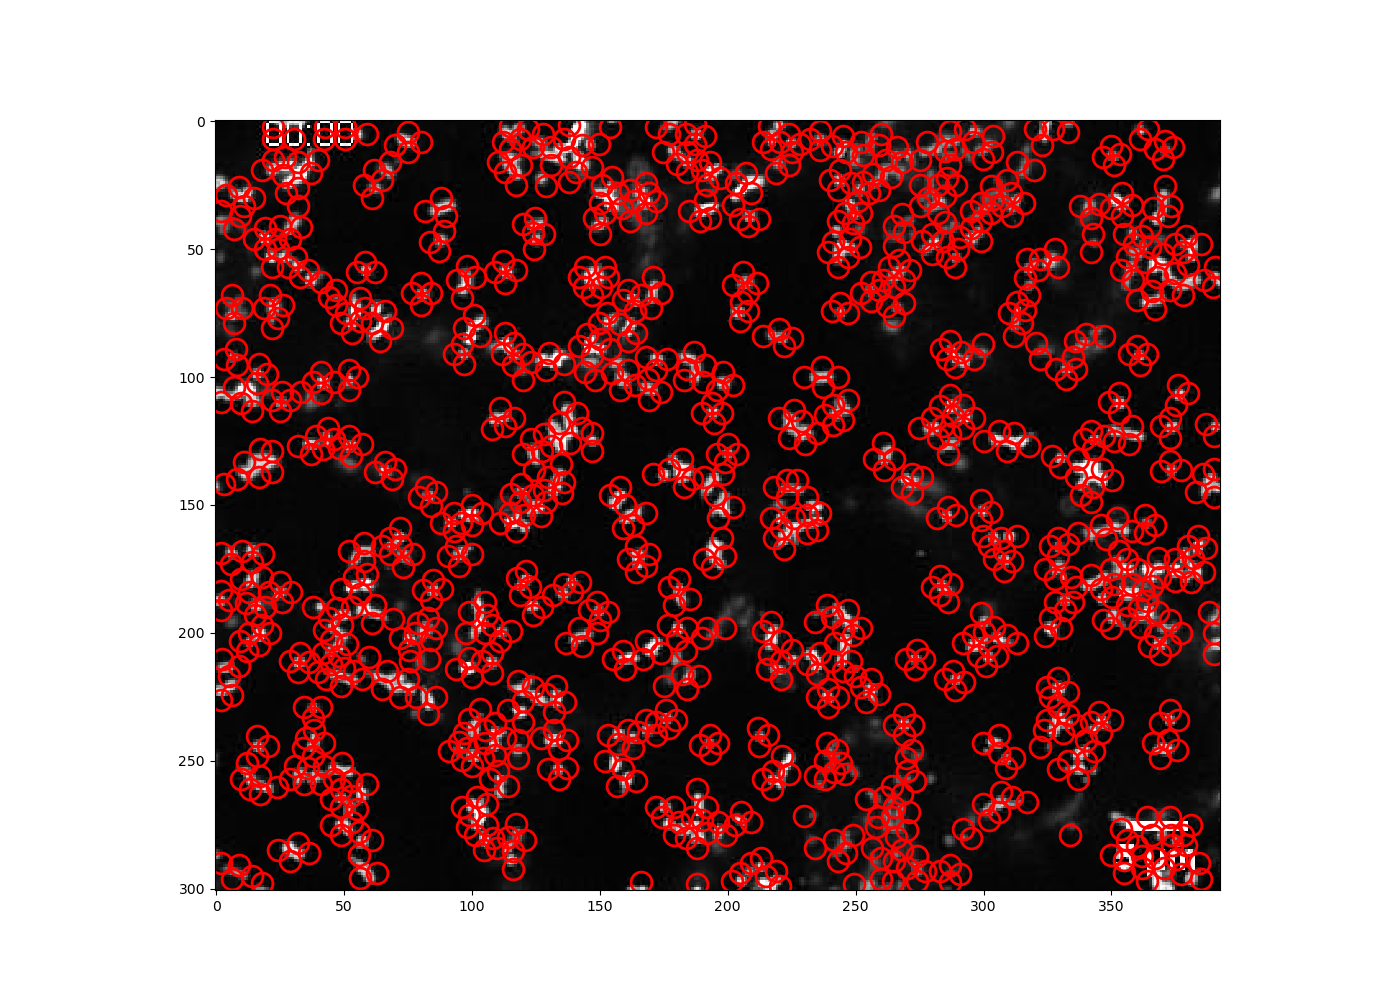
\includegraphics[scale=0.35]{Grafiken/trackpyBilder/locate(f0, diameter=3).png}
    \caption{Beispiel von Partikelerkennung mit Trackpy.}
    \label{fig:kap1_Trackpy_beispiel}
\end{figure}
	
In Anbetracht der Gesamtheit der Merkmale, die im Zusammenhang mit der Erwägung von Bibliotheken (Software), die zur Erreichung des oben genannten Ziels beitragen könnten, genannt wurden, ist \textbf{trackpy} der am besten geeignete Kandidat für unsere Arbeit. 

